\documentclass[10pt,a4paper]{article}
\usepackage[latin1]{inputenc}
\usepackage[english]{babel}
\usepackage{amsmath}
\usepackage{amsfonts}
\usepackage{amssymb}
\usepackage{makeidx}
\usepackage{graphicx}
\usepackage[left=2cm,right=2cm,top=2cm,bottom=2cm]{geometry}

\author{Anders Dall'Osso Teigset}
\title{Puffer mechanism}

\begin{document}
\maketitle
%Summary
\newpage
\section{Summary}
\newpage
\tableofcontents
\newpage
\section{Introduction}
A load break switch should be able to interrupt currents less or equal the maximum load current in a distribution system. When interrupting a current the two contacts which a switch consists of start separating producing a gap between each other. Normally the current is not interrupted by this and an electrical arc ignites and burns in the contact gap \cite{bib:HVEbreak}. The arc consists of plasma, which is a mixture of negative and positive ions as well as electrons. Due to the energy dissipation produced by the arc the temperature in the plasma is very high. The electrical conductivity of the plasma channel is dependent of the temperature produced by the arc. When a high current is flowing it is almost a perfect conductor, but at low temperatures the conductivity is much poorer.

An AC-current have a natural zero crossing, as the current approaches this point the arc will start cooling and extinguish if properly cooled at this point of the power cycle. The working principle of a switchgear is to cool the arc sufficiently when the current approaches zero and then quench the arc when the current is zero. At this moment the current is interrupted and a voltage builds up across the open contacts. This voltage is called the recovery voltage. The steepness and amplitude of the recovery voltage \cite{bib:HVEbreak} and the design of the switchgear will decide if a new arc ignites between the contacts after the current zero. If an arc re-ignites ether by a thermal or a dielectric breakdown the interruption has failed. 

Upon till now SF$_6$ and vacuum based technology have been dominating the compact medium-voltage switchgear market. Air insulated switchgear does exists but they are space consuming and are not applicable for use in a compact substation design. A compact substation is one of the most common designs for substations in the medium-voltage level of the distribution system. Figure \ref{fig:compact substation} displays a compact substation which can be used in the medium-voltage distribution system. The switchgear is a module that can be detached from the compact substation and removed trough its front panel. As figure \ref{fig:compact substation} shows there are a limited amount of space available for the switchgear. Therefore the main challenge for an air insulated switchgear design for this kind of application is set by the amount of space available in the compact substation.

\begin{figure} [h]
\centering
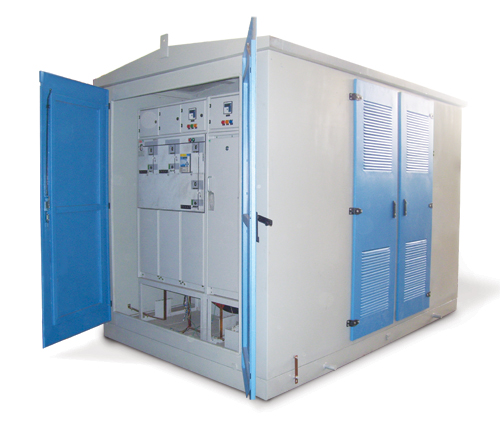
\includegraphics[scale=0.5]{Bilder/Introduction/general_substation.jpg}
\caption{Compact substation with open front panel} \label{fig:compact substation}
\end{figure}

The main choice of interrupting media in switchgear has been SF$_6$ since its discovery in the 1970ies. The gas exhibits many properties which is well suited for an isolation gas. It is highly electron negative which gives it good dielectric strength and arc-interrupting capabilities. The breakdown voltage of SF$_6$ is almost three times higher than air at atmospheric pressure \cite{bib:SF6PI}. It has excellent heat transfer properties as an interrupting medium \cite{bib:SF6PI}. The gas also reforms itself when dissociated under the high temperature conditions in an electrical arc. SF$_6$ produces no polymerization, carbon or other conductive deposits during arcing. It is also chemically compatible with most insulation materials and conductive materials \cite{bib:SF6PI}. The gas is also well suited for use in low temperature environments since its boiling point is fairly low even at high pressures. The gas in its stable form is nontoxic, non-flammable and non-explosive. It is also thermally stable and do not decompose at normal operating temperatures for a closed switch \cite{bib:SF6PI}. SF$_6$ based switchgear tends to be cheap to produce relative to other designs, and the gas itself is also affordable at today prices.


SF$_6$ have some disadvantages, when exposed to electrical discharge or arcing it forms highly toxic and corrosive compounds \cite{bib:SF6PI}. It is also hard to remove non-polar contaminants like air and its breakdown voltage is sensitive to water vapour and conductive particles. However it biggest downside is probably that it is an effective infrared absorber. This makes it a strong greenhouse gas \cite{bib:SF6PI} and it is regarded to be almost $20000$ times as potent as CO$_2$.

0.4 \% of the greenhouse gas emissions in Norway is due to SF$_6$ and is mainly used in switchgear or other high voltage equipment \cite{bib:KlimaKur2020}. In Norway the use of SF$_6$ is regulated through a voluntary contract between the environmental department and the end user, mainly the power companies \cite{bib:KlimaKur2020}. If a compatible air based switchgear design is released on the market it can be assumed that the power companies will be interested in the new technology. It is also possible that the government will restrict the use of SF$_6$ gas if the private sector do not follow the guidelines of the environmental department.

A prototype switch have been developed which allows adjustment of many design parameter such as nozzle and contact geometry, contact movement and gas pressure. The contacts consist of one female contact, or tulip and one male contact, or pin. The tulip is immovable, while the pin can be opened by a spring trigged by an electromagnet. Previous results have shown that most of the successful interruptions have occurred when the pin is outside the nozzle \cite{bib:CIAMVLBS}. Cold air simulations of the different geometries have shown that volumetric flow of air is much lower when the pin is inside the nozzle \cite{NOE}. The results from previous testing and cold air simulations might suggest that the pin is clogging the nozzle and preventing a good air flow. Therefore a new nozzle has been designed with a doughnut area, the area between the nozzle and the pin, which is bigger than the area of the pin. This is assumed to give a volumetric flow of air that is almost the same when the pin is inside the nozzle as well as outside. The theory has been verified by cold air simulations. However the clogging effect generated by an arc has not been taken into account and it is expected that this will have an impact on the volumetric flow.

Several different nozzle geometries are going to be tested and it is assumed that the chance for a successful current interruption inside the nozzle will be approximately the same as outside the nozzle. Since the size of the arc compared to the pin will vary between the different nozzle geometries and current amplitudes, a clogging effect is assumed to occur and might be revealed as an lower interruption success rate for certain geometries.

\newpage
\section{Theory}
\subsection{Switchgear design}
\subsubsection{General design}
\subsubsection{Prototype design}
\newpage
\subsection{Interrupting currents}
\subsubsection{The difference between air and SF$_6$ as interrupting medium}
\newpage
\subsection{Environmental impacts of SF$_6$ from electrical power industries}
\newpage

\begin{thebibliography}{10}


\bibitem{bib:HVEbreak} \textit{M. Runde}, \textit{Current Interruption in Power Grids}. Trondheim: Norwegian University of Science and Technology, 2013, p. 1-2 - 1-6

\bibitem{bib:SF6PI} \textit{L.G. Christophorou, J. K. Olthoff, and R.J. Van Brunt}, "\textit{Sulfur Hexafluoride and the Electric Power Industry}", \textit{IEEE Electrical Insulation Magazine, vol. 13, No. 5, pp. 20-24}, Oct. 1997.

\bibitem{bib:CIAMVLBS} \textit{E. Jonsson, N. S. Aanensen and M. Runde}, "\textit{Current Interruption in Air for a Medium Voltage Load Break Switch}", \textit{IEEE Trans. Power Delivery}, to be published.

\bibitem{bib:KlimaKur2020} "\textit{KLIMAKUR2020}", Oslo: Klima- og forurensningsdirektoratet, 2010, p. 197
\end{thebibliography}
\end{document}